\documentclass[11pt]{article}

\usepackage{graphicx}
\usepackage{mathtools}
\usepackage{amssymb}
\usepackage{titlesec}
\usepackage{hyperref}
\usepackage{varioref}
\usepackage{listings}
\usepackage{mathrsfs}
\usepackage{algorithm}
\usepackage{algpseudocode}
\usepackage[a4paper, total={6in, 9.5in}, footnotesep=2\baselineskip]{geometry}
\usepackage[font=small,labelfont=bf,skip=2pt]{caption}
\usepackage[toc,page]{appendix}
\usepackage{enumitem}
\usepackage{array}
\usepackage{multirow}
\usepackage{float}
\usepackage{placeins}
\usepackage{color}
\usepackage{graphics}
\usepackage[utf8]{inputenc}
\usepackage{mdframed}

% parameters for \maketitle
%\title{Computational Vision Lab 01 - Introduction to Matlab}
%\author{Johannes Heidecke}

% paragraph formatting
%\setlength{\parindent}{2em}
%\setlength{\parskip}{2em}
\renewcommand{\baselinestretch}{1.1}

% prevent orphans and widows
\widowpenalty10000
\clubpenalty10000

\begin{document}

\begin{titlepage}

\vspace*{\fill}

\newcommand{\HRule}{\rule{\linewidth}{0.5mm}} % Defines a new command for the horizontal lines, change thickness here

\center % Center everything on the page
 
%----------------------------------------------------------------------------------------
%	HEADING SECTIONS
%----------------------------------------------------------------------------------------

\textsc{\LARGE Universitat Politècnica de Catalunya}\\[0.5cm] % Name of your university/college
\textsc{\LARGE Universitat de Barcelona}\\[0.5cm] % Name of your university/college
\textsc{\LARGE Universitat Rovira i Virgili}\\[1.5cm] % Name of your university/college
\textsc{\Large Master in Artificial Intelligence}\\[0.5cm] % Major heading such as course name
\textsc{\large Computational Vision}\\[0.5cm] % Minor heading such as course title

%----------------------------------------------------------------------------------------
%	TITLE SECTION
%----------------------------------------------------------------------------------------

\HRule \\[0.4cm]
{\huge \bfseries Edges and Contours}\\[0.4cm] % Title of your document
\HRule \\[1.5cm]
 
%----------------------------------------------------------------------------------------
%	AUTHOR SECTION
%----------------------------------------------------------------------------------------

\Large \emph{Authors:}\\
Johannes \textsc{Heidecke}\\
Alejandro \textsc{Suárez Hernández}\\[3cm]

%----------------------------------------------------------------------------------------
%	DATE SECTION
%----------------------------------------------------------------------------------------

{\large October 2016}\\[3cm] % Date, change the \today to a set date if you want to be precise

\vspace*{\fill} % Fill the rest of the page with whitespace

\end{titlepage}


\tableofcontents
\listoffigures

\clearpage

\section{Exercise 1: Haar-like features and classification}

\subsection{Compute and visualize Haar-like features}

{\bfseries
Question 1:
\begin{itemize}
\item Explain the obtained 2-dimensional plot on the feature space.
\item Given this 2-dimensional plot, can we infer the defined Haar-like features
			are appropriate for face/non-face discrimination?
\end{itemize}}

\subsecion{Classification in the feature space}

{\bfseries Question 2: \\Is the result good enough? Explain your response}

{\bfseries Question 3: \\What do you infer from the figure? Explain your response}
\section{Mean-shift segmentation}

The algorithm is not deterministic because at each update step the next
point to update (i.e. move towards the mean of its neighbourhood
centered in that point) is selected randomly. This is done in the 
line 47 of the provided \texttt{MeanShiftCluster.m} file
(\texttt{tempInd = ceil( (numInitPts-1e-6)*rand);}).
This also means that two executions of the Mean-shift algorithm do
not yield necessarily the same value
(unless the seed of the random generator is fixed).
\section{Question 3}

{\bfseries Try to slowly increase or decrease the (peak) threshold. Comment
why the number of detected keypoints decreases when the threshold is increased.
Is this the expected behavior according to the way the threshold is defined?}


Figure \ref{fig:n_peak_thresh} shows the effects of increasing the peak threshold on the number of detected keypoints. For a threshold value of 0, 1816 keypoints are detected. For a threshold of 0.005, the number decreases to 1698. The number of keypoints keeps decreasing monotonously until it reaches 2 for a threshold of 0.09 and finally 0 for a threshold of 0.1.
\begin{figure}[!hbt]
  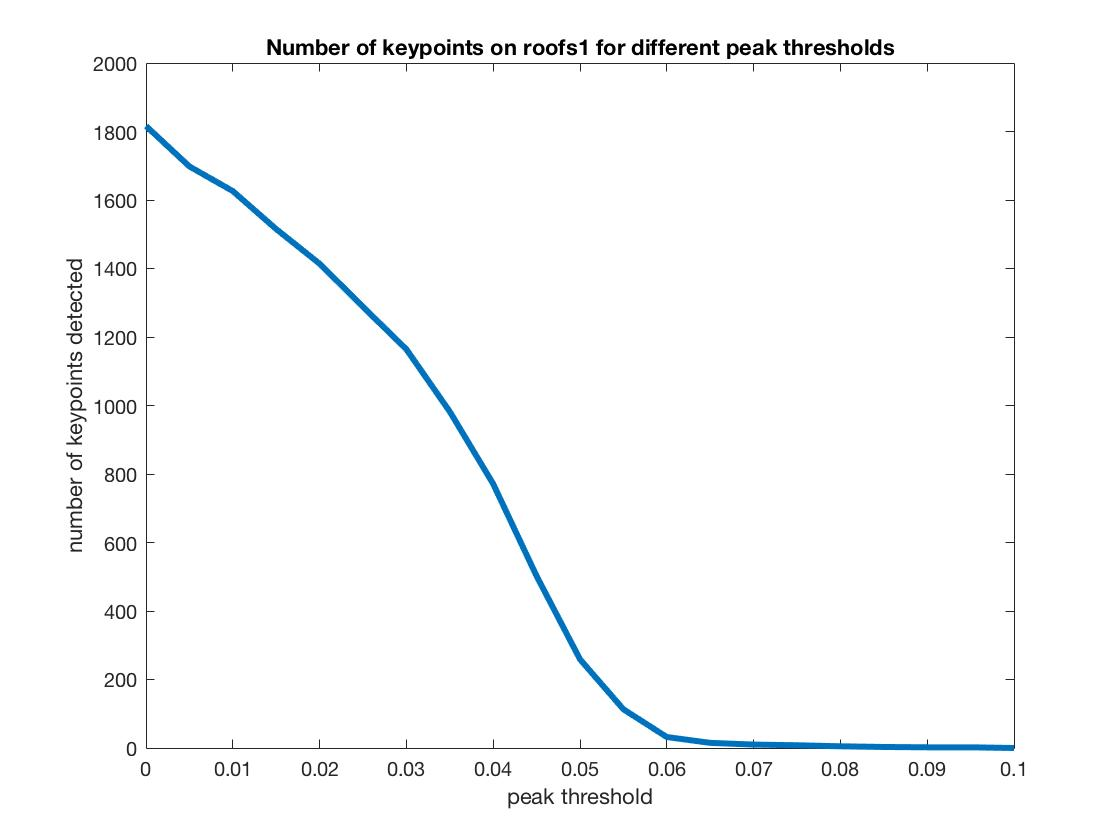
\includegraphics[width=\textwidth]{img/n_peak_thresh}
  \caption{Relationship between peak threshold and number of detected keypoints}
  \label{fig:n_peak_thresh}
\end{figure}

The number of detected keypoints decreases when increasing the threshold, since more and more keypoints with low extreme values of the difference of Gaussian in the scale space are filtered out, until finally there are none left. The peak threshold leads to the behavior we would expect. 

\begin{figure}[!hbt]
  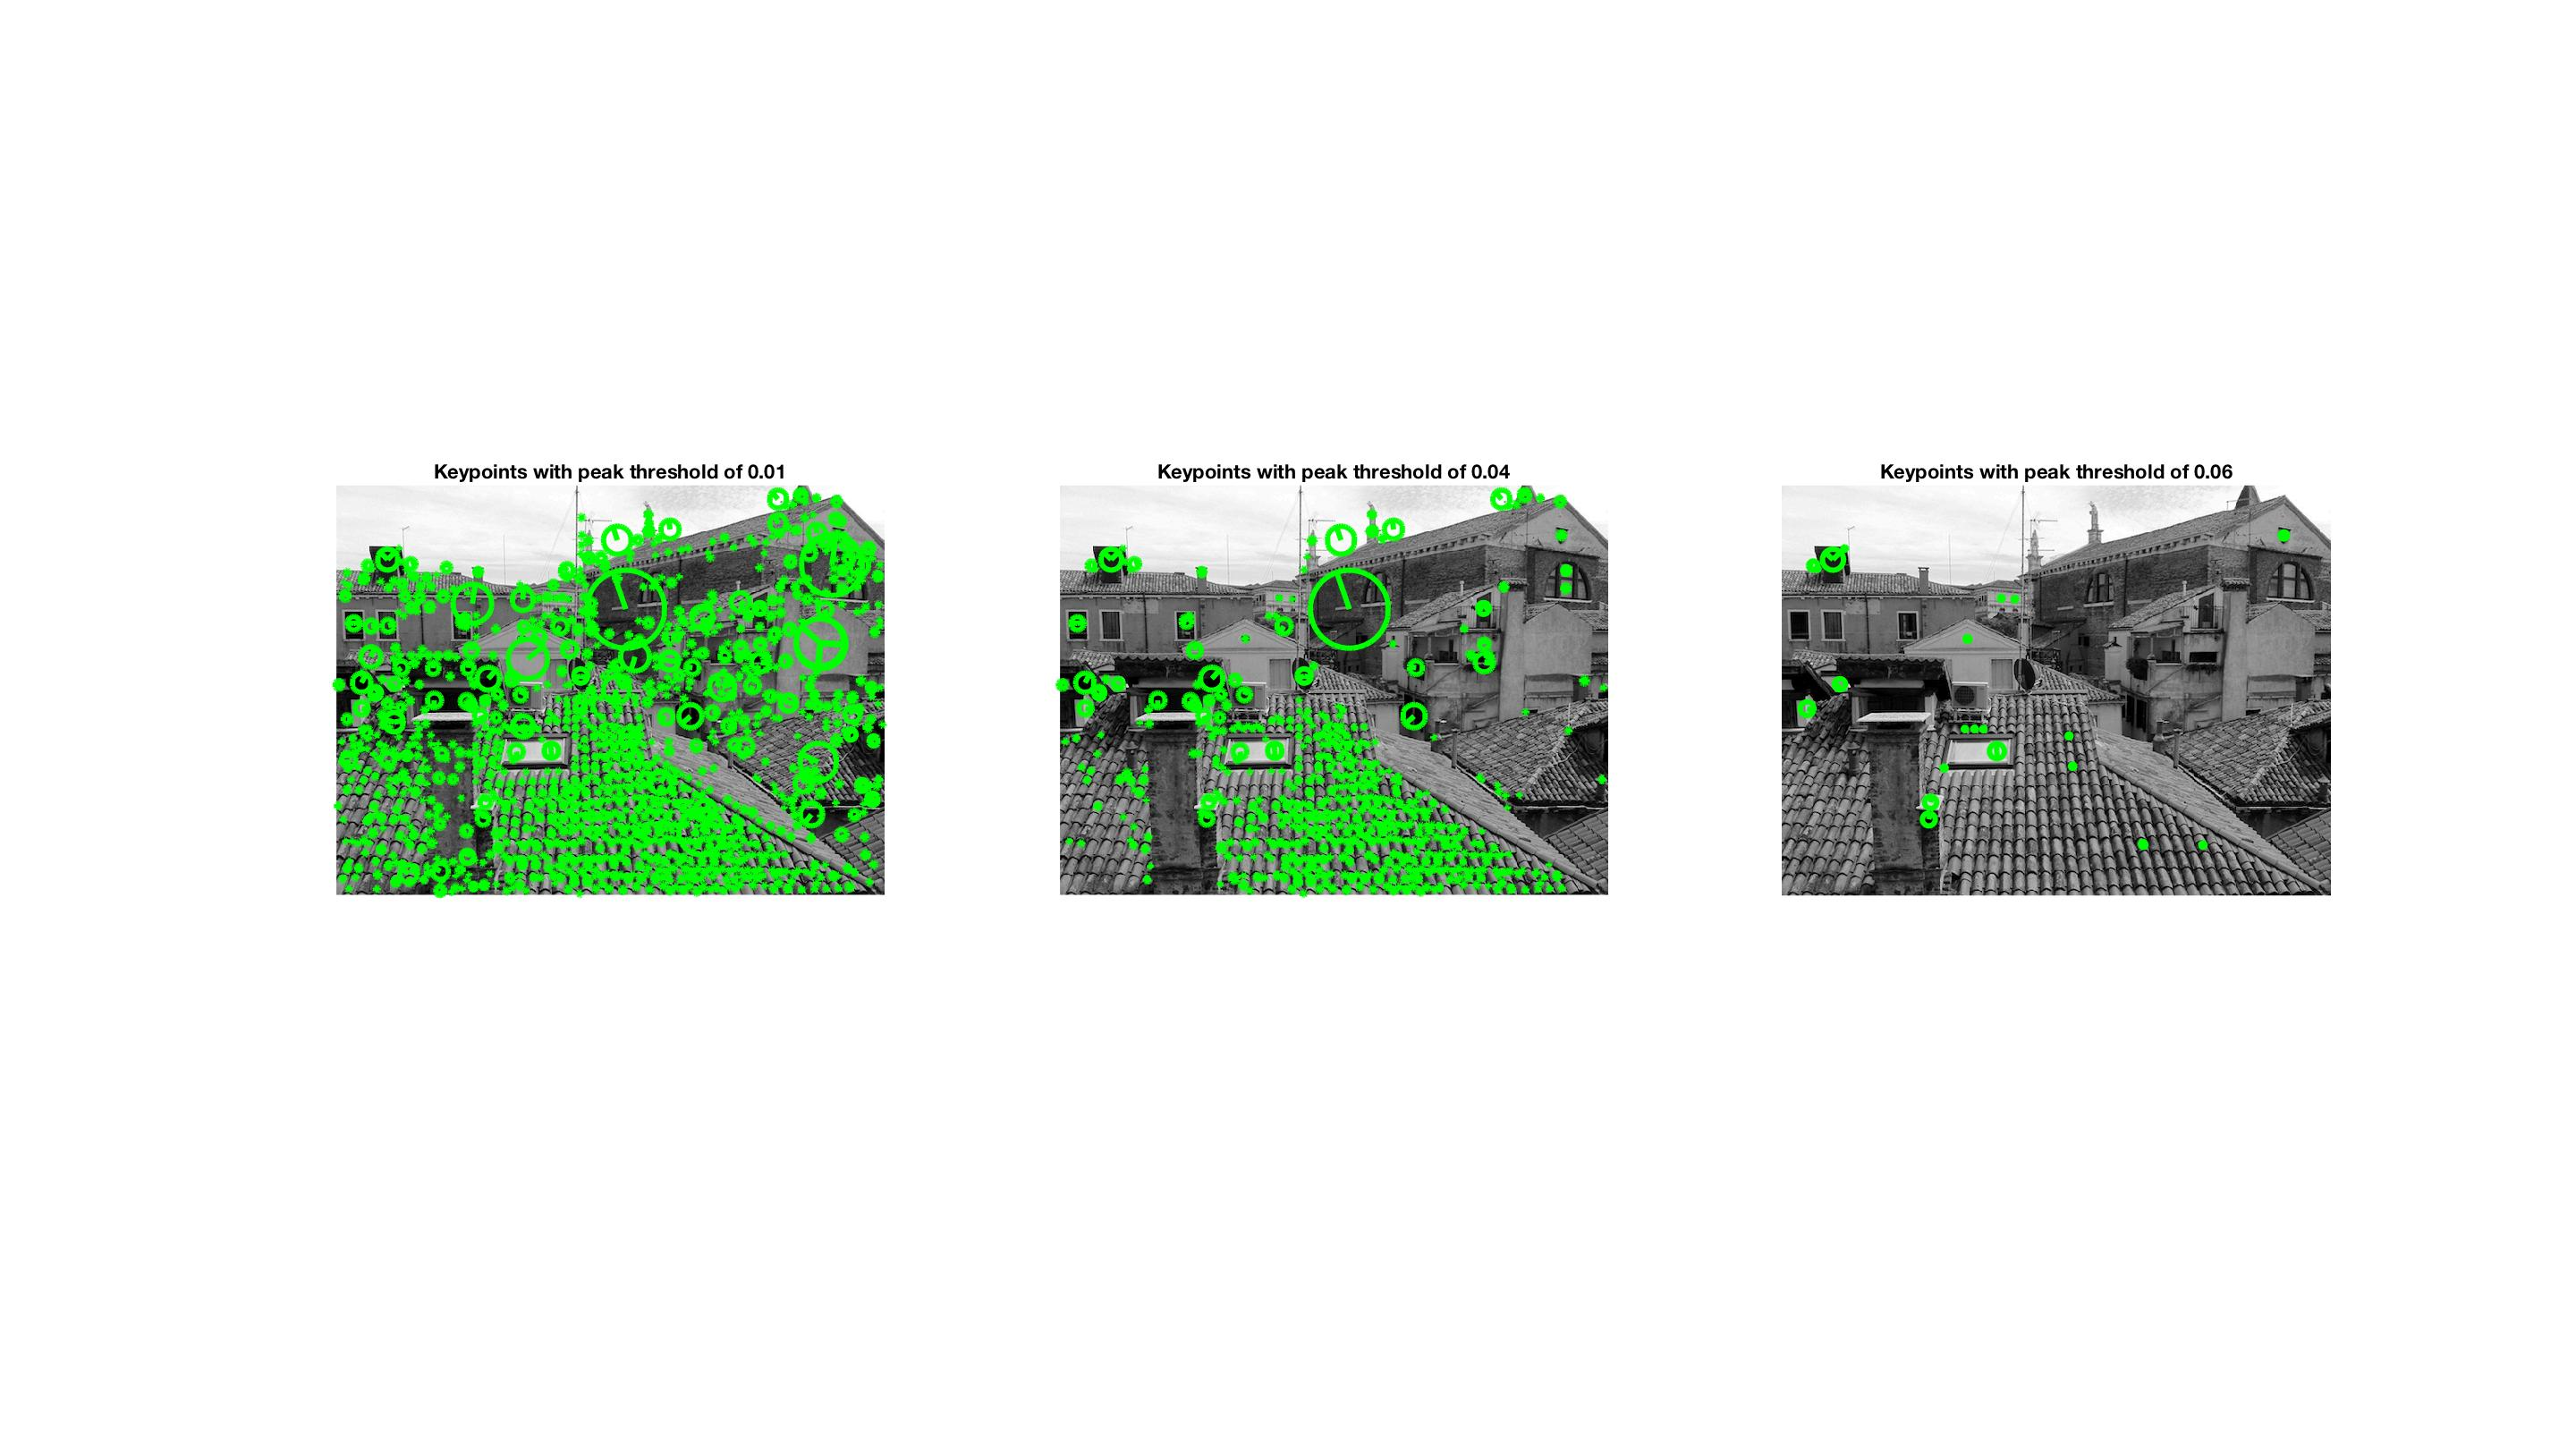
\includegraphics[width=\textwidth]{img/inc_peak_thresh}
  \caption{Effects of increasing the peak threshold}
  \label{fig:inc_peak_thresh}
\end{figure}

Figure \ref{fig:inc_peak_thresh} shows the effects of increasing the peak threshold on the example image \texttt{roofs1}. Keypoints in areas with low contrast and thus low extrema are sorted out first. For a threshold of 0.01 keypoints in the low contrast sky almost entirely are sorted out. For a threshold of 0.04, keypoints on the roof tiles begin to disappear. For a threshold of 0.06 only a few keypoints in very distinct positions remain.

\newpage
\section{Question 4}

{\bfseries Try to slowly increase or decrease the (edge) threshold. Comment
why the number of detected keypoints decreases when the threshold is decreased.
Is this the expected behavior according to the way the threshold is defined?}

The edge threshold is used to filter out extrema of the difference of Gaussians that lie on an edge, i.e. that have a small curvature. Keypoints on edges can be moved along the edges with minor differences in their features and are thus not well suited to be selected. Figure \ref{fig:inc_edge_thresh} shows the effects of different levels of edge thresholds on the keypoints that are detected.

\begin{figure}[!hbt]
  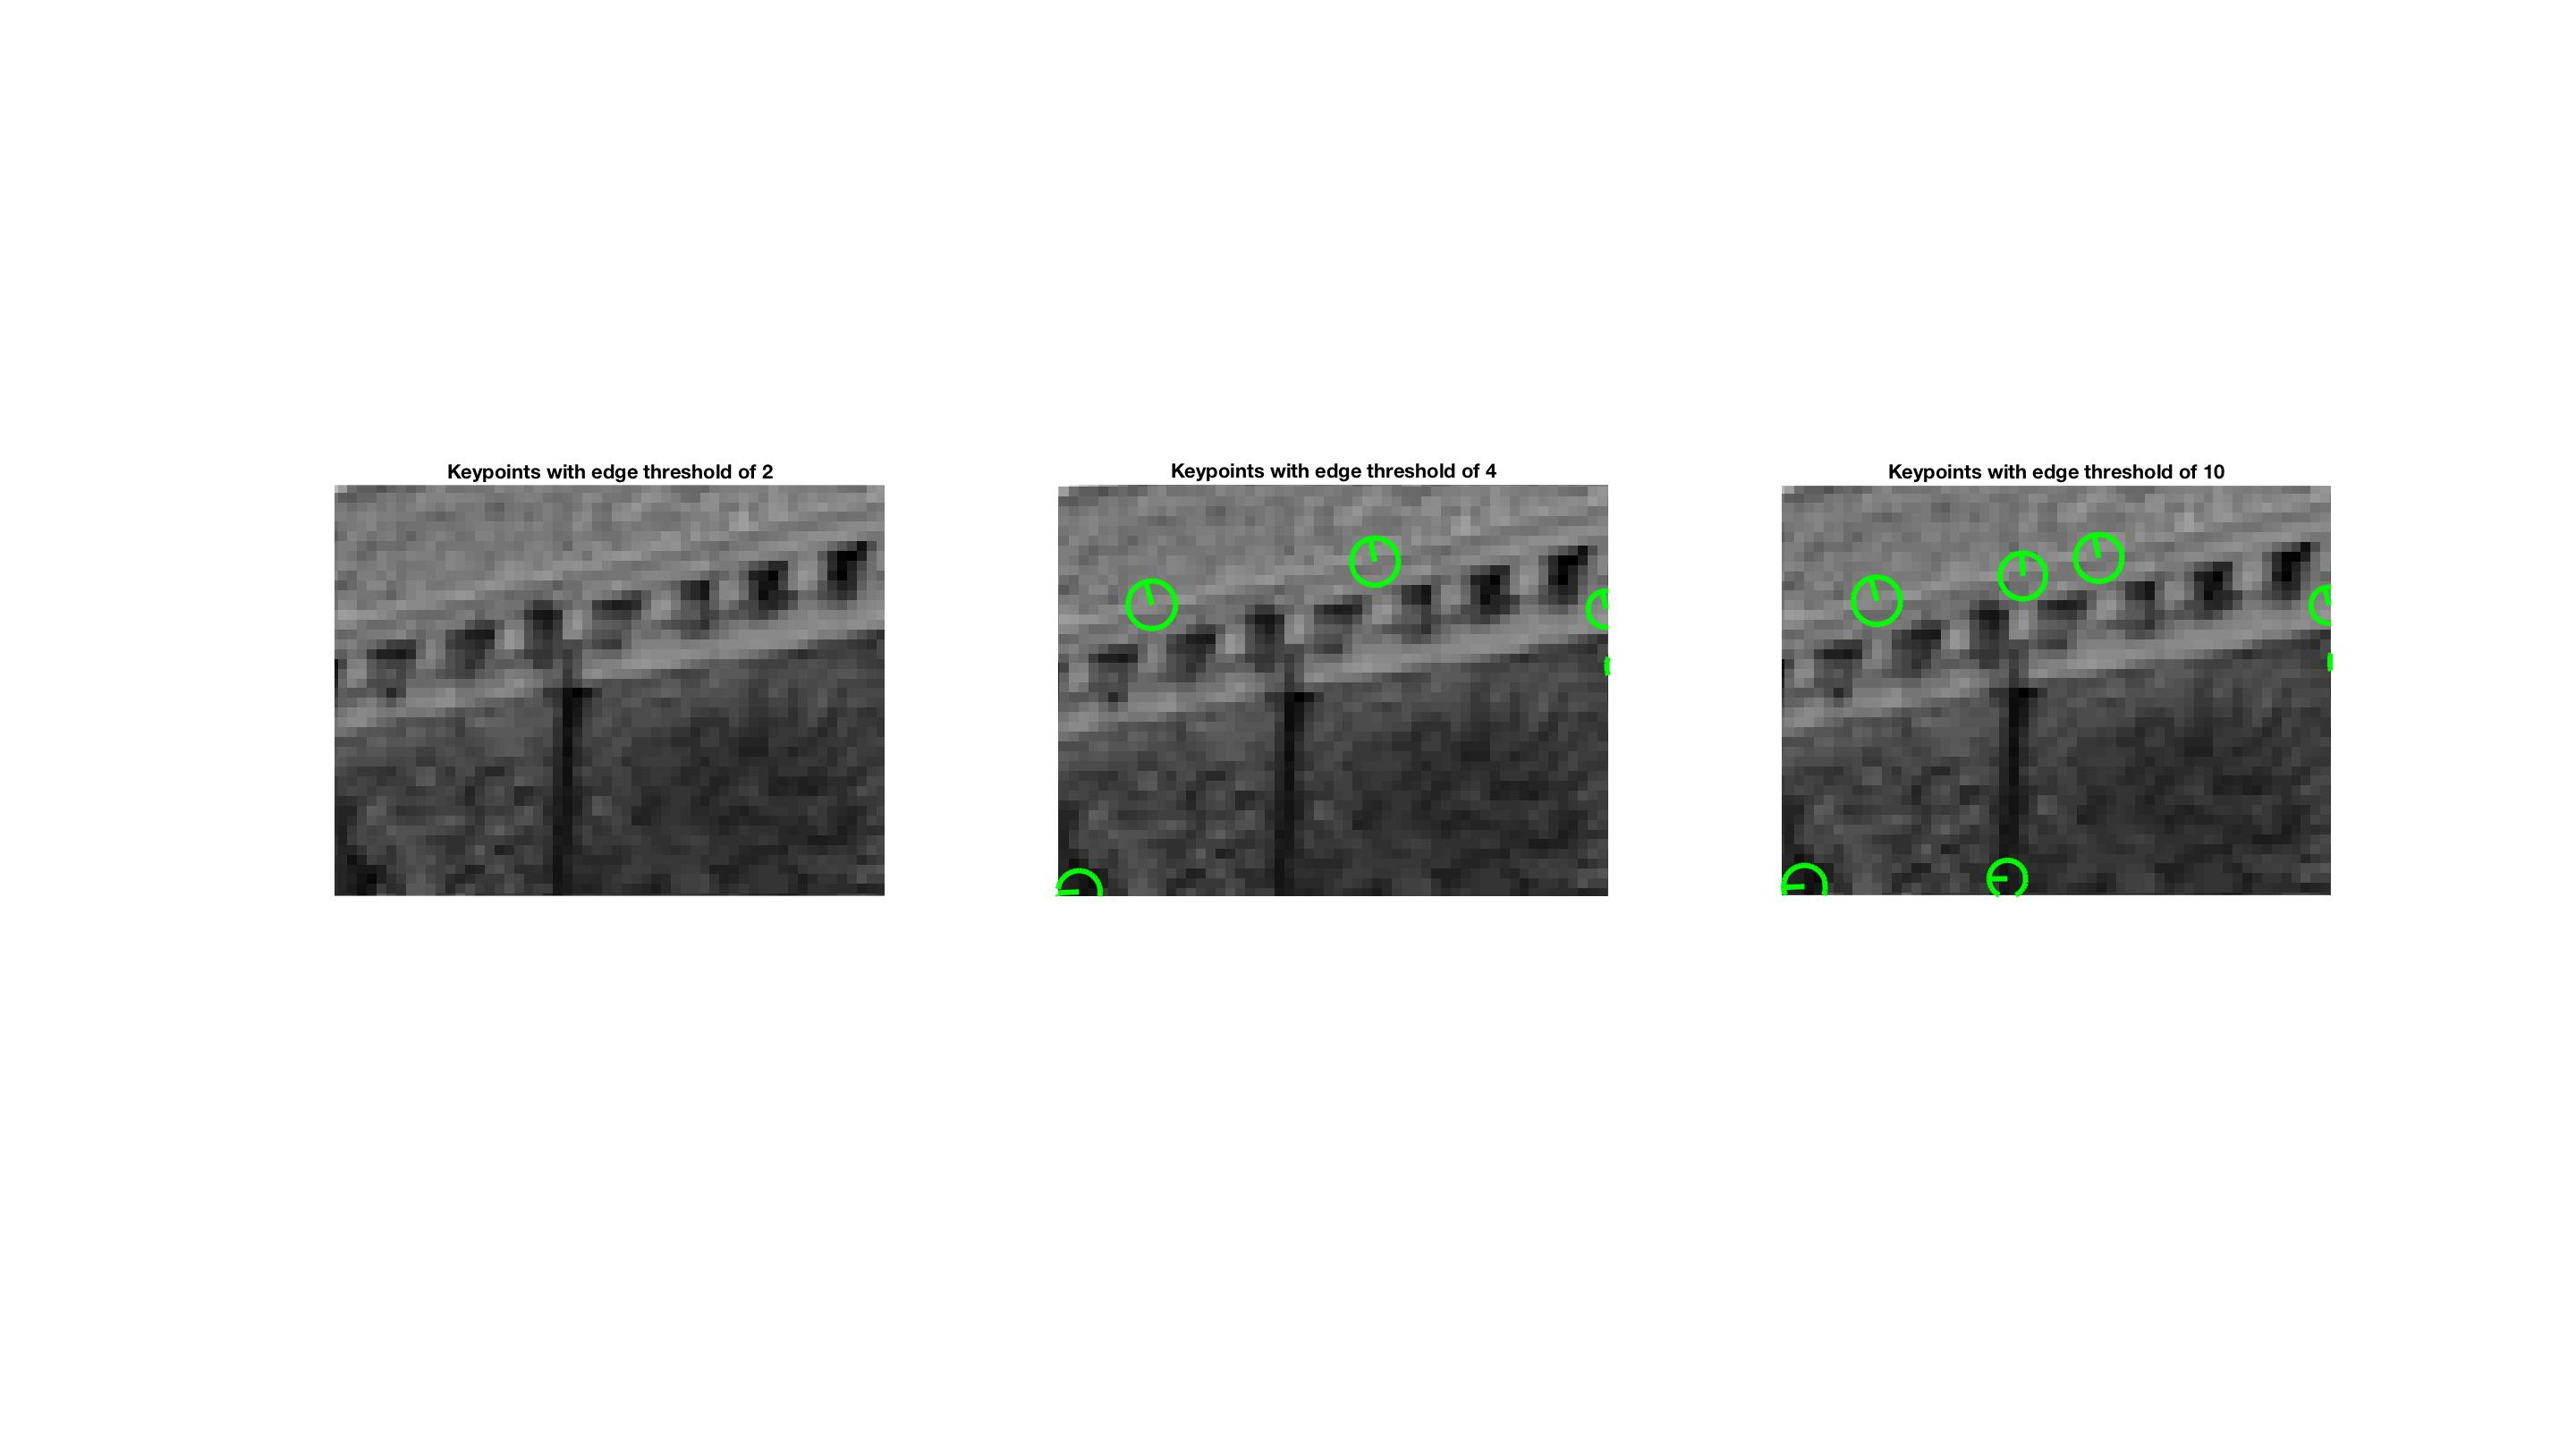
\includegraphics[width=\textwidth]{img/inc_edge_thresh}
  \caption{Effects of decreasing the edge threshold}
  \label{fig:inc_edge_thresh}
\end{figure}

As we can see in figure \ref{fig:inc_edge_thresh}, low values of the edge threshold effectively remove keypoints that lie along edges. The edge threshold r is the ratio between the largest magnitude eigenvalue $ \lambda_{max} $ and the smaller one $ \lambda_{min} $ with $ \lambda_{max} = r \lambda_{min} $. A small r means that both eigenvalues are relatively close to each other, which indicates a high curvature. With decreasing $ r $ we remove more and more keypoints on edges. This effect can be observed in figure \ref{fig:n_peak_thresh}: While there are no keypoints with a ratio $ r $ that is exactly 1, for increasing the edge threshold we allow more and more keypoints that lie on increasingly obvious edges. This fits to our expected behavior based on the way the threshold is defined. 

\begin{figure}[!hbt]
  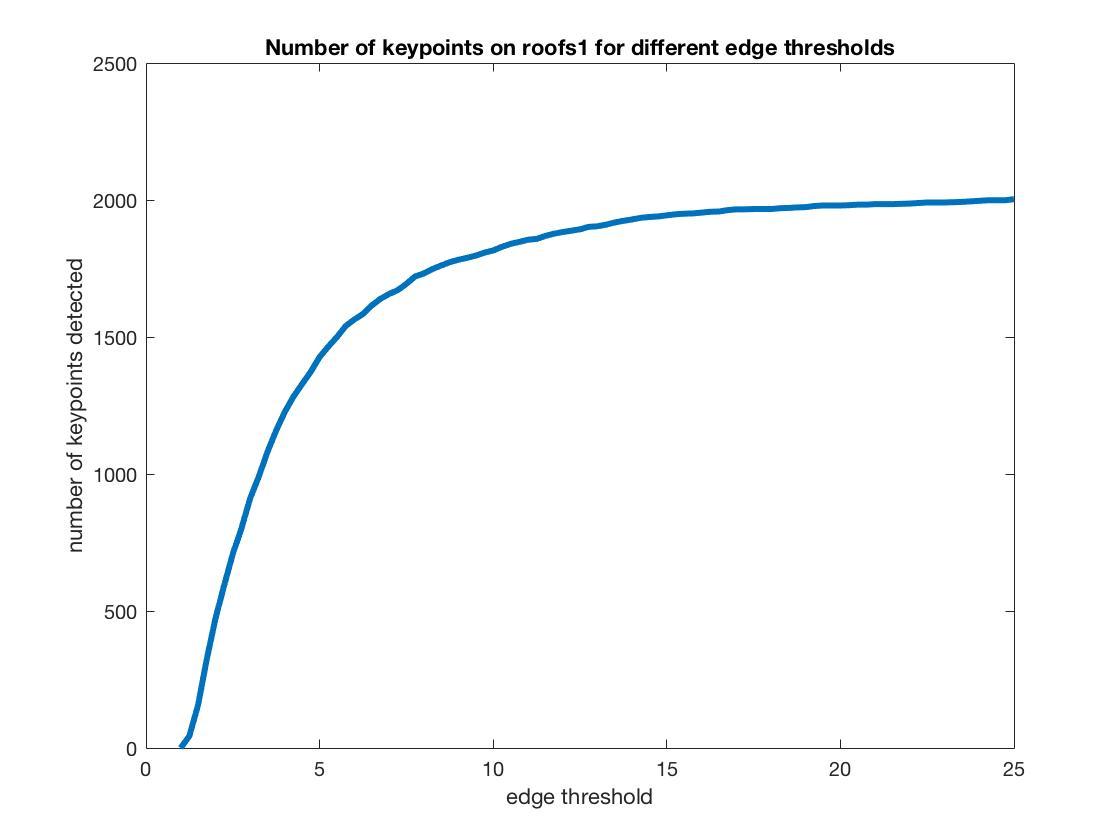
\includegraphics[width=\textwidth]{img/n_edge_thresh}
  \caption{Relationship between edge threshold and number of detected keypoints}
  \label{fig:n_peak_thresh}
\end{figure}


\section{Image binarization}

The built-in Matlab function \textit{imbinarize} creates a logical array for an grayscale image I given a threshold t in which all pixels with values above t get mapped to a 1 and all other pixels to a 0.

Figure \ref{fig:task19} shows binarizations for a gray scale image of a car for different thresholds. It can be seen that the optimum threshold depends heavily on the specific image. In this case, a threshold of 20 or 30 still maps most pixel to white values and does not yield a useful result. When moving the threshold closer to 1, most pixels get mapped to a white output, as the in the first image of figure \ref{fig:task19}. Conversely, for very high thresholds (like the extreme 255) maps almost every pixel to black.

\begin{figure}[!hbt]
  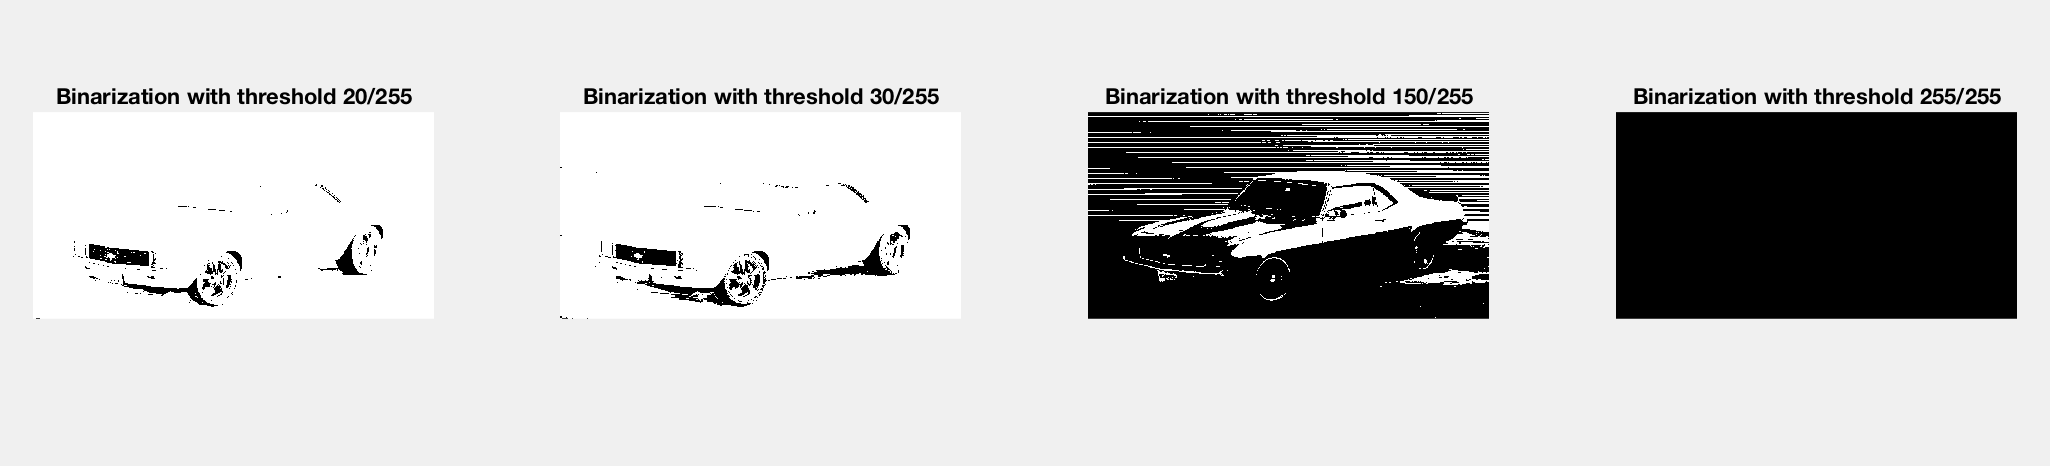
\includegraphics[width=\textwidth]{./img/task19.png}
  \caption{Image binarization with different thresholds}
  \label{fig:task19}
\end{figure}

Figure \ref{fig:task20} shows the pixel-wise product of the original image and its binarization with a threshold of 150/255.

\begin{figure}[!hbt]
  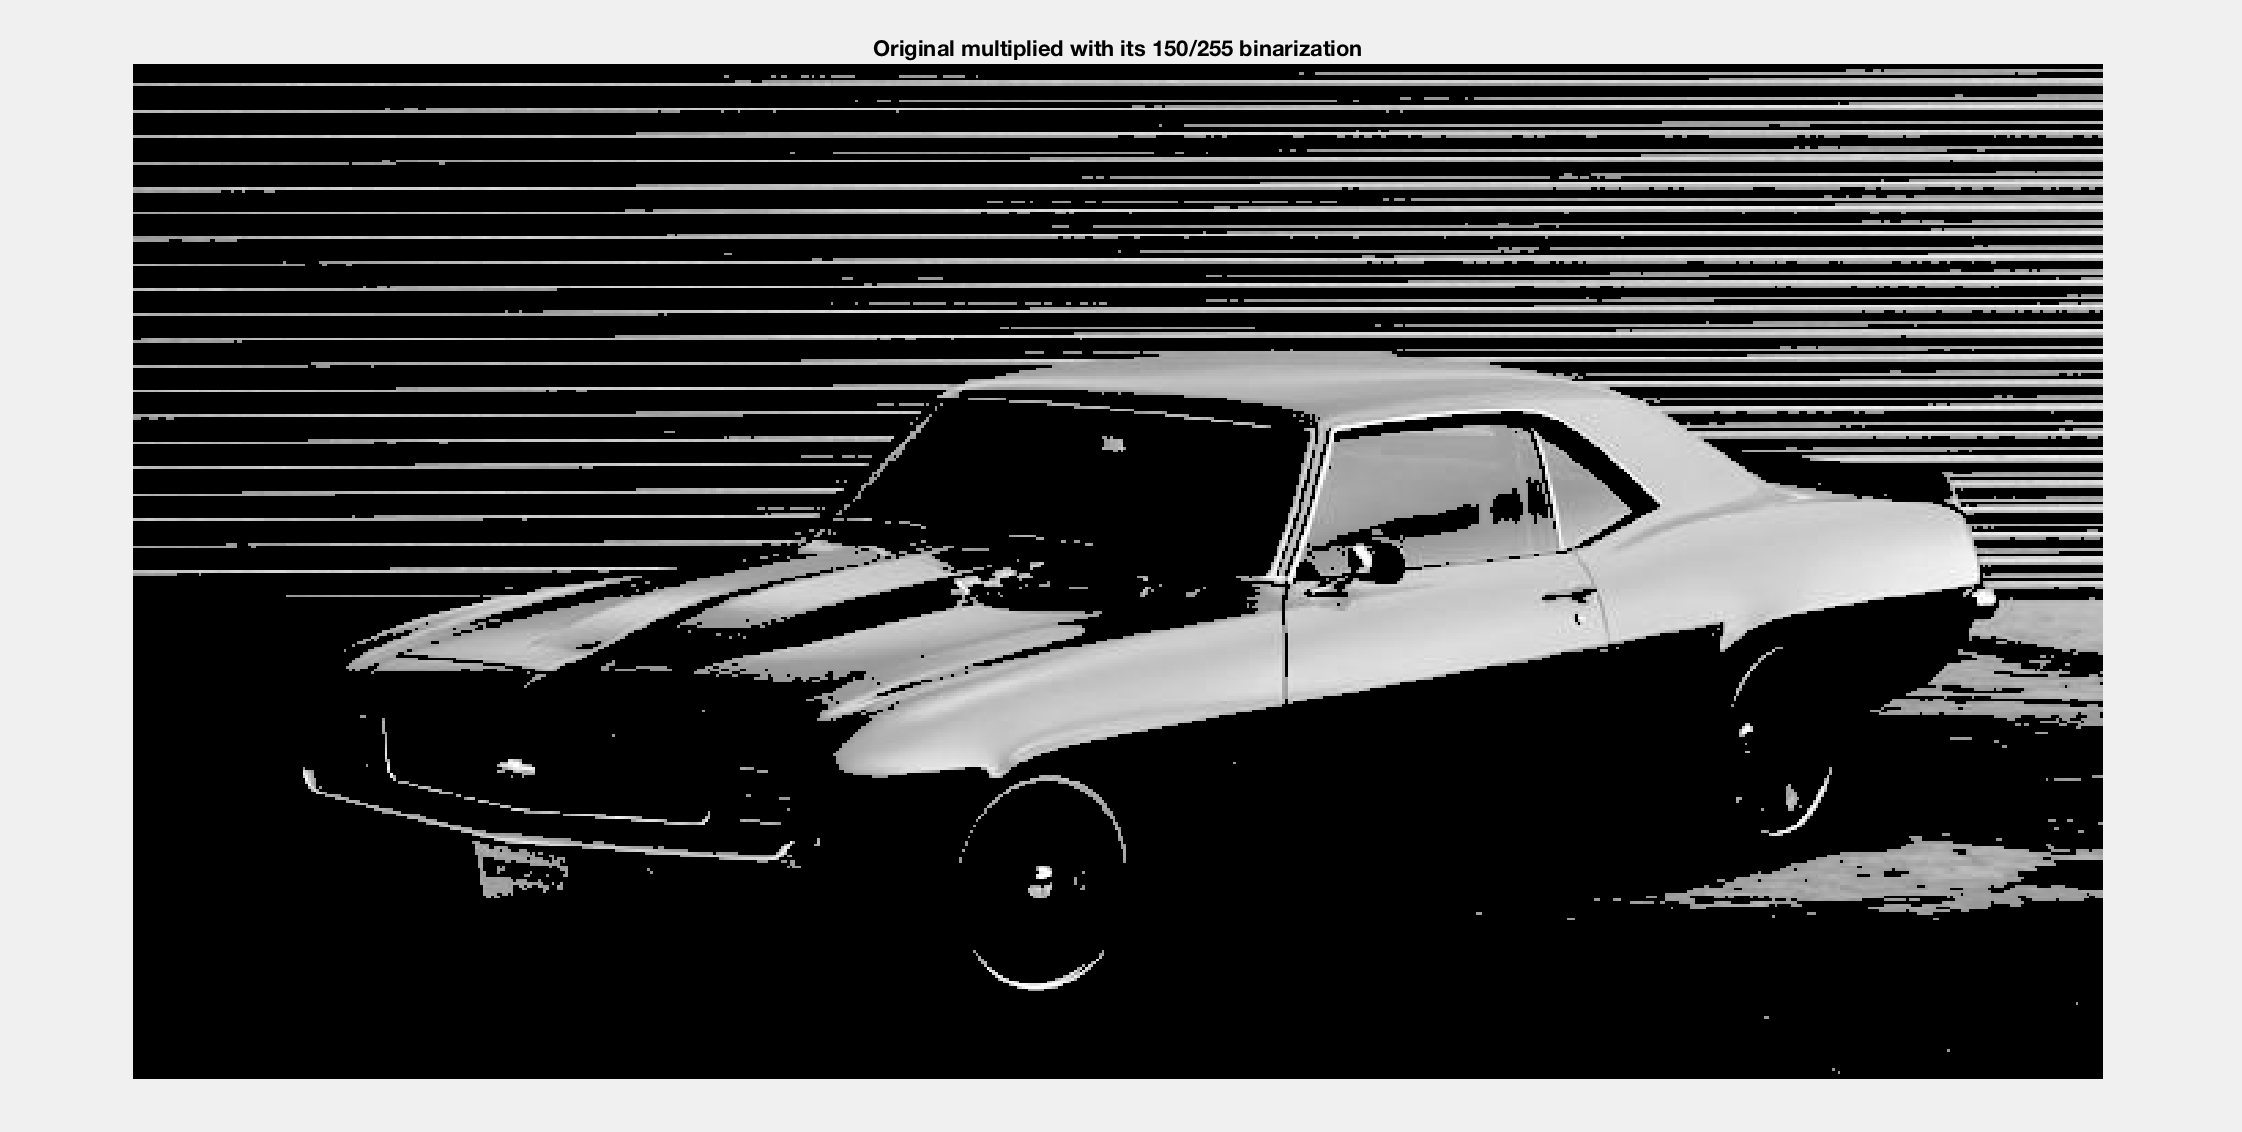
\includegraphics[width=\textwidth]{./img/task20.png}
  \caption{Original multiplied with its binarization}
  \label{fig:task20}
\end{figure}

Figure \ref{fig:task21} shows the pixel-wise product of the original image and its inverted binarization with a threshold of 150/255.

\begin{figure}[!hbt]
  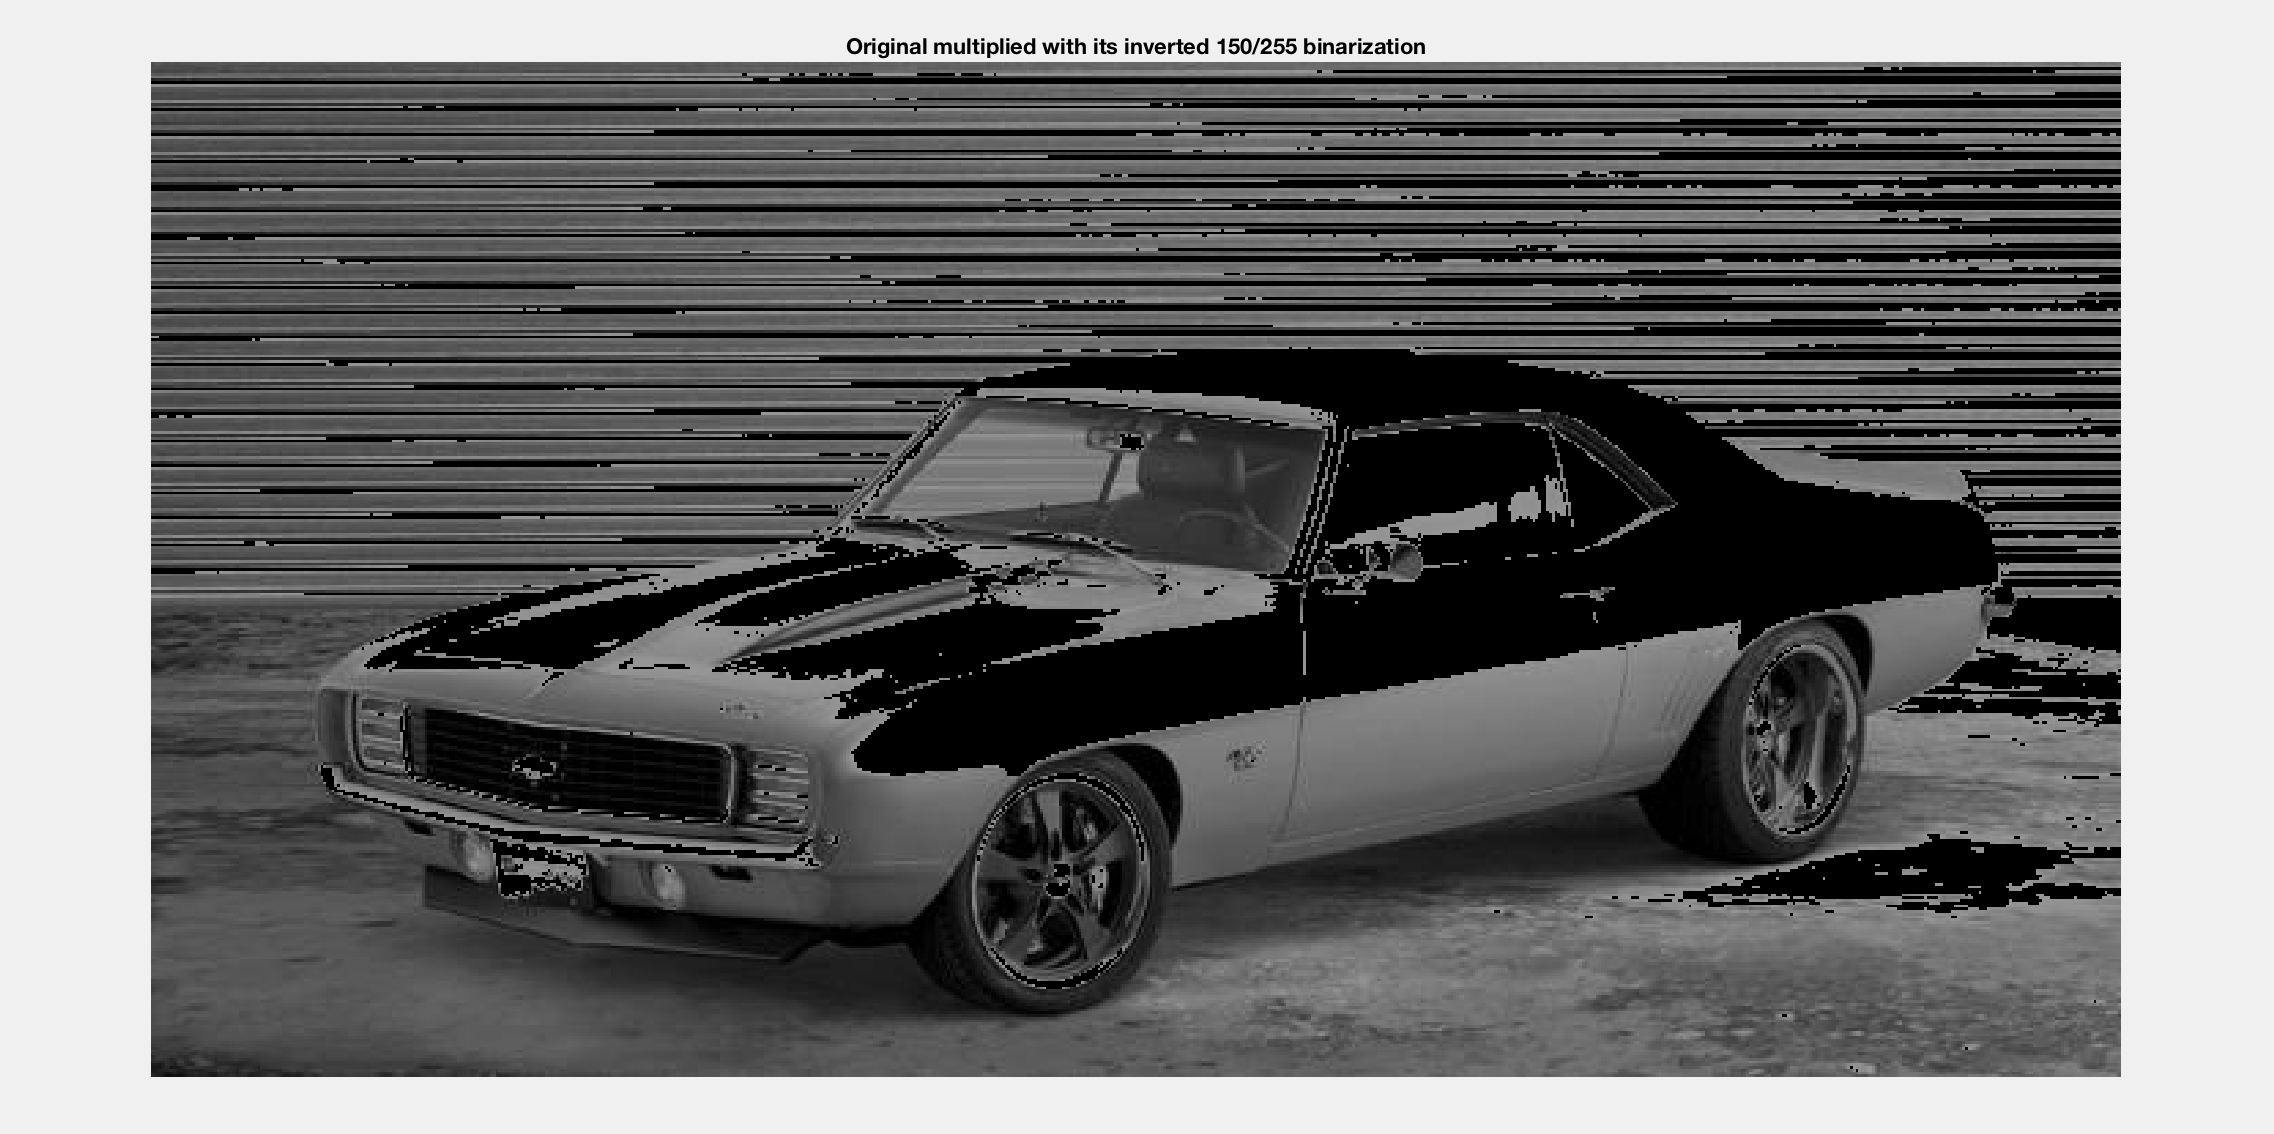
\includegraphics[width=\textwidth]{./img/task21.png}
  \caption{Original multiplied with its inverted binarization}
  \label{fig:task21}
\end{figure}
\section{Treating color images}

In exercise 6, the pixels showing the hand are separated from the black background of the original image and copied onto a second image. The commands used for this process can be found in \texttt{exercise6.m}. The resulting image is depicted in figure \ref{fig:task22}.

\begin{figure}[!hbt]
  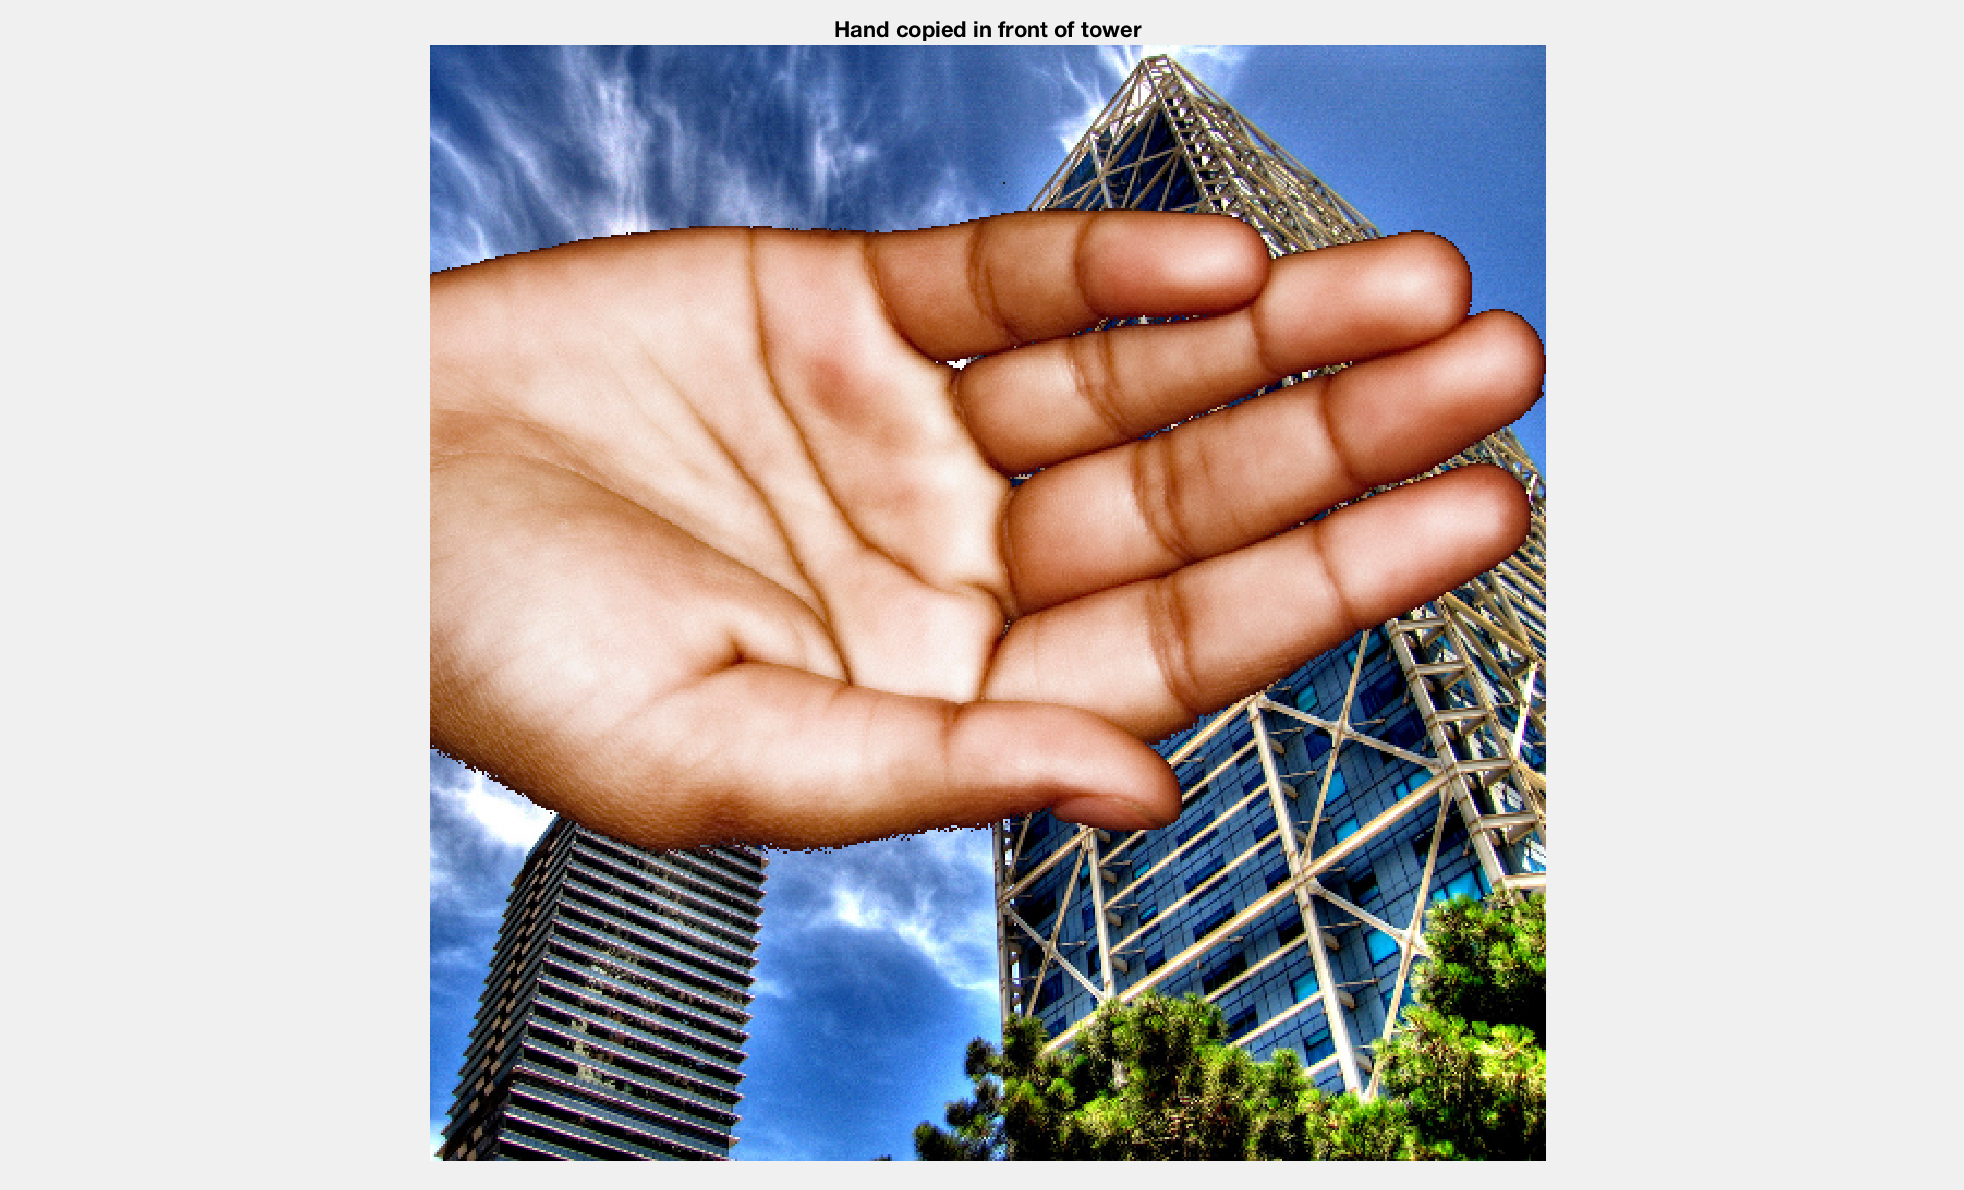
\includegraphics[width=\textwidth]{./img/task22.png}
  \caption{Hand copied in front of tower}
  \label{fig:task22}
\end{figure}

\clearpage
\begin{appendices}
\section{Delivered code files}

Here we list all the delivered script and function files delivered for this practice.
We include relevant observations. For full insight, we refer the reader to the
source code.

\begin{itemize}
	\item \texttt{exercise1.m}
	\item \texttt{exercise2.m}
	\item \texttt{exercise3.m}
	\item \texttt{exercise4.m}
	\item \texttt{exercise5.m}
	\item \texttt{exercise6.m}
\end{itemize}

\end{appendices}

\end{document}
